\documentclass[border=3pt]{standalone}
\usepackage{tikz}
\usetikzlibrary{arrows.meta,calc}
\tikzset{pin/.style={-{Stealth[length=5pt]}},
  blk/.style={draw, thick, minimum width=16mm, minimum height=18mm, font=\sffamily}}
\begin{document}
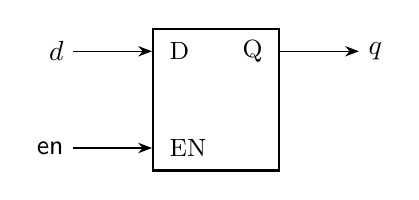
\begin{tikzpicture}[font=\sffamily]
  \node[blk] (l) {};
  \node[anchor=west, font=\small] at ($(l.north west)+(1mm,-3mm)$) {D};
  \node[anchor=west, font=\small] at ($(l.south west)+(1mm,3mm)$) {EN};
  \node[anchor=east, font=\small] at ($(l.north east)+(-1mm,-3mm)$) {Q};
  \draw[pin] ($(l.north west)+(-10mm,-3mm)$) node[left]{$d$} -- ($(l.north west)+(0,-3mm)$);
  \draw[pin] ($(l.south west)+(-10mm,3mm)$) node[left]{en} -- ($(l.south west)+(0,3mm)$);
  \draw[pin] ($(l.north east)+(0,-3mm)$) -- ++(10mm,0) node[right]{$q$};
\end{tikzpicture}
\end{document}
